%\sectskip
\section{Principles for Layer Design}
\label{sec:seq:design}
%\asectskip

Our layered framework  provides an elegant formalism for decomposing
the verification of a complex kernel into a large number of tractable
tasks: we design a series of certified abstraction layers, which serve
as increasingly deep specifications for an increasing portion
of the kernel code.  These abstract layers are designed in a way such
that complex interdependent kernel components are untangled and
converted into a well-organized kernel-object stack with clean
specification.  In this section, we present the layer design process
and common principles we have followed in our development.


\paragraph{Principle 1: introduce layers to reflect dependencies between kernel modules} One purpose 
of layers is to enforce code isolation and abstraction.
When a module $M$ depends on another module $N$,  
abstraction layers should be organized in such a way that
$M$ can be reasoned about in terms of an abstracted version of $N$.

For example, since the virtual memory management code relies on physical memory management,
the code which performs allocation and
deallocation of physical pages in terms of allocation tables
is first abstracted into a layer object (\cf Figures~\ref{fig:alt}-\ref{fig:palloc:spec}).
This object provides the primitives \code{palloc} and \code{pfree} to operate on an abstract allocation
table \code{AT}.
Then functions such as \code{pt\_insert} and \code{ pt\_rmv}, which manipulate
page mappings at the virtual memory management level,
can be verified with a more
abstract view of the allocation
table, without worrying about its concrete memory representation and code
implementation.
On the other hand, if two kernel modules mutually depend on each other,
they have to be introduced within a single layer.

\ignore{
\paragraph{Principle 2: introduce a layer when the abstraction of kernel object changes}
(I am not sure whether this principle should be explicitly listed here or not -- Ronghui)

[Speculation by jeremie, try and add examples:]
On occasion,
it might be useful to offer multiple views of a single kernel object
at different levels of abstraction.
For instance,
in cases where there is a very large gap between
the concrete data structures used by a layer object and
the abstract description we ultimately want to use,
it can be simpler to decompose the refinement proof in two steps
by introducing an intermediate representation
which is already somewhat abstracted,
but similar in structure to the concrete implementation.
More over,
client code in different parts of the kernel
might be better understood with different levels of abstraction
for their kernel object. [Is that true? example?]

In such cases,
we can introduce a new layer which does not add any code and layer objects,
but simply changes the abstraction level of the existing ones.
}

\paragraph{Principle 2: introduce layers to
lift the memory accessors}
OS kernels must manage limited physical memory and
provide contiguous address spaces
for high-level kernel modules and user programs.
Because much of the code assumes that 
the memory management sets up the virtual address space properly,
initialization has been a sticking point
in previous verification efforts~\cite{klein2009sel4, vaynberg12},
in which the virtual address space setup is either not verified,
or verified separately as an external lemma.
We address this issue by introducing the memory accessors in the abstraction layers.

Based on the CompCert memory model,
we equip the  semantics of LAsm with notions of \emph{page fault} and \emph{address translation} provided by the layer interface $L$.
The memory accessors of a layer $L$
specify how memory loads and stores are carried out
in terms of the system description at that level of abstraction.
Those accessors are implemented by the physical and virtual memory management components,
 organize memory in terms of various \emph{units} (byte, page, address space),
and provide different addressing modes and protection mechanisms.
Because our kernel code is compiled using CompCertX,
its own stack frames and static data have to be modeled as independent blocks.
\ignore{However, as explained in Section~\ref{sec:base:memm},
we prove that user programs can never access
the kernel portion of the address space.}
We use an external tool~\cite{veristack}
to prove that the stack usage of our compiled kernel is bounded
such that stack overflows cannot occur:
the computed bound is much less than the dedicated 4K bytes we use
for kernel stacks.

Integrating the various views of the memory into our layered approach
allows us to reason about memory accesses in the same way that
we reason about other kernel services:
as long as the low-level memory accessors
as configured by our kernel code,
contextually refine more abstract memory accessors,
any code we can write and reason about in terms of the latter
can be shown to have an equivalent behavior
when run on top of the former.



\ignore{
Based on the physical memory model (Fig.~\ref{fig:spec:memmodel}(a)), we can verify the \emph{physical memory management}, 
which will provide a different view over the memory (Fig.~\ref{fig:spec:memmodel}(b)).
The physical memory will be organized as pages,
and a page is accessible only after it has been allocated.

Relied on this paged physical memory model,
 the \emph{virtual memory management} will provide a
stronger protection over the memory and set up the virtual address space 
(Fig.~\ref{fig:spec:memmodel}(c)). When paging is enabled,
all the memory accesses are forced to do address translation with page map.
Thanks to this virtual address memory model, 
we can prove the memory isolation properties
\ronghui{which will be discussed in David's Section}.
}


\paragraph{Principle 3: introduce a layer when a stronger invariant needs to be proved}
Each  layer interface specifies a predicate
on the memory and the abstract states.
This invariant is satisfied by the initial state, and
preserved by memory accessors and layer primitives.
It therefore holds in all client contexts,
at any point of execution.

In previous verification efforts,
proving invariants has typically been challenging.
For example, in seL4, the thread queues are implemented as doubly-linked lists with 
the following invariant:
\begin{invariant}
\label{inv:spec:queue}
 All back links in thread queues point to appropriate nodes and all elements point
 to thread control blocks.
\end{invariant}
Proving this invariant is difficult
for several reasons.
As stated in ~\cite{klein2009sel4}:
\begin{quote}
  Invariants are expensive because
  they need to be proved not only locally,
  but for the whole kernel ---
  we have to show that no other pointer manipulation in the kernel
  accidentally destroys the list or its properties.
  [\ldots]
  The treatment of globals becomes especially difficult
  if the invariants are temporarily violated.
  For example,
  adding a new node to a doubly-linked list
  temporarily violates invariants that the list is well formed.
\end{quote}
However, in our layered approach,
we do not need to establish the invariant in a single step.
We first introduce a layer to introduce
an abstract thread queue object,
and hide the concrete queue representations
in the memory (via CompCert memory permissions).
Therefore, the remaining kernel code cannot access
the corresponding memory blocks directly.
Moreover, since the queue operations 
are replaced by  layer primitives,
there is no longer a point in the execution
at which the invariants have to be temporarily violated.
\ignore{Finally, some complex invariants are implied by
the correspondence with our abstract representations.
For instance, in our setting, Inv.~\ref{inv:spec:queue} 
naturally follows from the contextual refinement between
concrete thread queues and
abstract ``thread list'' objects.


After paging is enabled, both kernel modules and user processes
run in a virtual address space.
To ensure the correctness of these kernel modules and user processes on top of virtual memory
management, we require the following invariants to hold:
\begin{invariant}
\label{inv:seq:virtual}
1) paging is enabled only after the initialization of virtual memory management;
2) the memory regions that store kernel-specific data must have the kernel-only 
permission in all page maps;
3) the page map used by the kernel is an identity map
4) the non-shared parts of user processes' memory are isolated.
\end{invariant}

Invariant~\ref{inv:seq:virtual} no longer holds 
if the privileged primitive that sets the \code{CR3}
register is present in the layer, as the unknown context code may write
an invalid address into \code{CR3} using the provided primitive. To solve this issue, another
layer is introduced with a wrapper function that takes the process id as argument,
instead of an actual address. Then the function sets \code{CR3} to the
starting address of the predefined corresponding process's page table structure.
The primitive that directly sets the \code{CR3} register is hidden from the
new layer, and the invariants are introduced in the new layer.
This is one of the rare cases where performance overhead is introduced
(one extra function call due to the wrapper).
It should be possible to use CompCertX's function-inlining optimization
to remove this overhead (this is left as future work).}

\ignore{
To prove this invariant, we have to introduce a new layer and add a wrapper
to the assembly function that modifies the value of \verb"CR3" register 
(which stores the staring point of page map).
Since the arbitrary call to this privilege assembly instruction is not safe,
this wrapper will first check whether the source pointer points to a page map that
satisfies the invariant. 

In this way, code rewritten is involved and a performance overhead is introduced.
To make this overhead less significant, we introduce a well-formed page map pool
object \verb"PMap" and the \verb"CR3" register is allowed to be modified only through
one primitive of \code{PMap}, which will store the starting
point of page maps within the pool to \verb"CR3". The overhead of this run time check is acceptable \ronghui{refer to the performance test}.
}

\paragraph{Principle 4: introduce a layer to facilitate initialization proofs}
To verify the initialization procedure of the kernel,
we introduce 
a special initialization primitive,
and an  initialization flag in the layer interface.
This logical initialization flag 
is \code{false} in the initial state and is set to \code{true} by the initialization 
primitive. Most of the invariants and
non-initialization primitives require as a precondition that
the initialization flag is \code{true}.
This guarantees that the initialization primitive is the first primitive that is executed. 

The initialization primitive can be
passed through from the layer below,
or a new one can be defined which extends that of the layer below
so as to initialize the new layer's data.
When a new layer object is introduced, 
we can create a new layer to initialize its abstract data to an appropriate state.
In the context of an operating system kernel, initialization functions are
relatively complex. Introducing an extra layer allows us to
avoid directly reasoning over the concrete memory. 
With this new layer, an initialization
function is verified using a more abstract specification.

\ignore{
Since each layer only have one explicit initialization primitive, when
the newly introduced layer objects need to be initialized,
we have to introduce a new abstract layer and a new initialization primitive. 
This new initialization primitive will first invoke the lower-level one
and then initialize the additional layer objects.
In this way, there is a initialization call chain from the top layer to 
the bottom layer.
}
\ignore{
\subsection{Defining abstraction layers}

Our framework specifies an abstraction layer
using five components:
a collection of objects,
a memory model,
an invariant which the memory and objects satisfy
at any point of the execution,
an initialization flag,
and an initialization primitive.
These five components define a logical view of
a subset of the kernel code
and extend our language with
an abstract specification of that code.
On top of this logical view, more code is introduced and
verified.

\paragraph{Layer objects}
\begin{figure}
\begin{center}
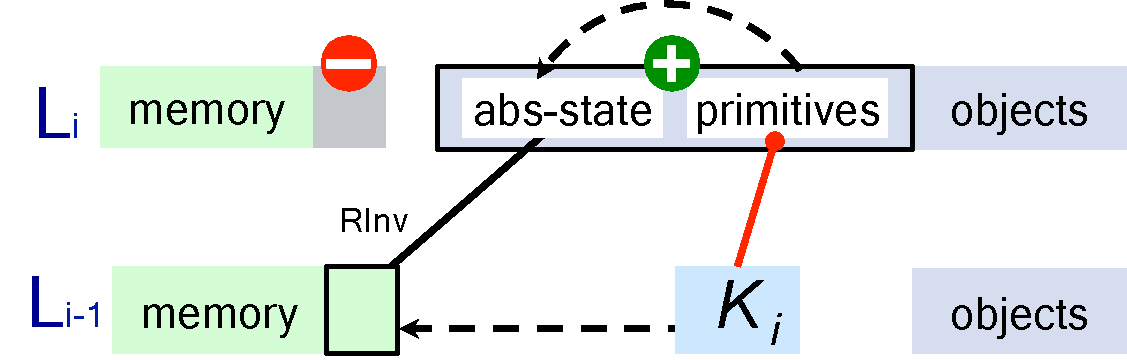
\includegraphics[scale=0.35]{figs/object}
\vspace*{-8pt}	
\end{center}
\caption{Introduce layer object}
\label{fig:spec:object}
\vspace*{-10pt}
\end{figure}

The layer objects are logical abstractions of kernel modules. 
In Fig.~\ref{fig:spec:object},
each layer object provides a set of abstract
states (which are abstractions of the module's private memory)
and a set of primitives (which are abstractions of the module's
interface specified in terms of the abstract states).
Consecutive layers may reuse some of the same objects,
introduce new layer objects by verifying additional code,
or hide some low-level objects
which are used to implement new objects but need not be
exposed to higher layers. Hiding unnecessary objects
facilitates invariant proofs since we can often use
stronger invariants at higher layers that would otherwise 
be violated by low-level objects.

For example, thread queues are implemented as doubly-linked lists
in \mCTOS{}, and the concrete implementations of the functions that
manipulate queues ({\it enqueue} and
{\it dequeue}) directly manipulate these doubly-linked lists in memory.
On the other hand, in our abstract queue layer object, a queue
is just a simple list of thread identifiers, and 
the {\it enqueue} and {\it dequeue} primitives are
specified directly over the abstract lists.
The contextual refinement relation between
the two layers (one with concrete implementation and the other
with the abstract layer object) ensures that any kernel/user context code
(e.g., the scheduler) running on top of the more abstract layer retains an
equivalent behavior when it is running on top of the layer with corresponding
concrete implementation.

As shown in Fig.~\ref{fig:spec:object},
to establish the contextual refinement relation
between concrete memory and abstract state,
we use Compcert memory permissions~\cite{leroy08} at the higher layer
to prevent the context code
from accessing the module's private memory.
Note that these permissions do \emph{not}
correspond to a physical protection mechanism,
but instead are entirely logical:
they ensure that the higher-level abstract machine
gets stuck whenever it executes
code that directly accesses this private memory.
By proving our kernel is safe (it does not get stuck),
we guarantee that this situation will not happen.

\begin{figure*}[th]
$$
\begin{array}{c|c}
\begin{array}{cc}
(a) &\hspace{-5mm} 
      \begin{array}{c}
			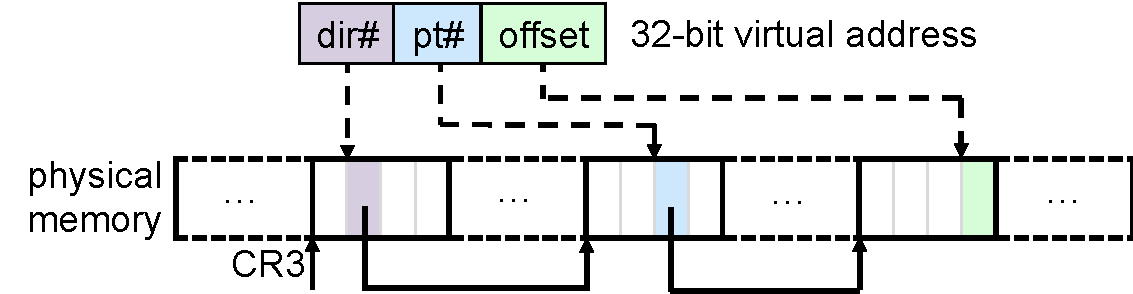
\includegraphics[scale=.4]{figs/mem_model_1} 
		\end{array}
\end{array}
& 
\begin{array}{cc}
(b) & \hspace{-5mm} 
\begin{array}{c}
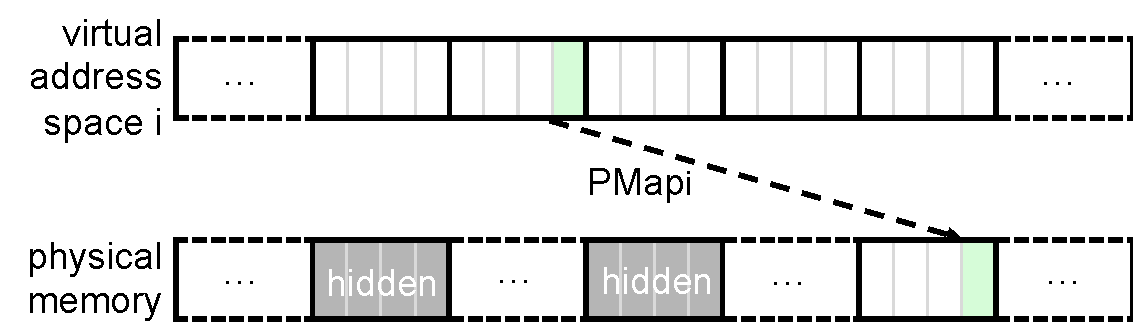
\includegraphics[scale=.4]{figs/mem_model_2}
\end{array}
\end{array}
\vspace*{-14pt}
\end{array}
$$
\caption{(a) machine memory model; (b) abstract memory model}
\label{fig:spec:memmodel}
\vspace*{-10pt}
\end{figure*}

\paragraph{Memory models} 



As shown in Fig.~\ref{fig:spec:memmodel}(a),
the \emph{machine memory model} is an unstructured CompCert memory block,
which is consistent with the hardware view of the physical memory.
Accesses to this memory block are
modeled in a way that mirrors the operation of the paging hardware.
By contrast,
in the top-level memory model (which we call the \emph{abstract memory model}),
address translation cannot be disabled; memory accessors operate on the basis of
the high-level, abstract descriptions of address spaces
rather than concrete page directories and page tables stored in the memory
itself (see Fig.~\ref{fig:spec:memmodel}(b)).


In the \emph{machine memory model}, when paging is enabled, each memory
access is accompanied by a two level page table walk starting from the
address stored in the \code{CR3} register, shown in Fig.~\ref{fig:spec:memmodel}(a). Switches of page tables are
performed by storing the top address of the other page table structure
into \code{CR3}.
In the \emph{abstract memory model}, we associate with each process a logical
partial map from a virtual address to a pair of physical address and
permission. The address translations are performed using the logical
mappings of the currently-running process, shown in Fig.~\ref{fig:spec:memmodel}(b).
With this high level memory model, some complex properties like
memory isolation can be proved more easily
(see Sec.~\ref{security}).

\mCTOSbase{} uses an additional intermediate memory model.
The \mCTOShyper{} extension presented in Sec.~\ref{sec:adapt}
uses yet another, virtualization-related model.
We introduce a new layer whenever we switch
from one memory model to another
and establish the contextual refinement between them.
\ignore{
A slightly more abstract version of this memory model,
the \emph{paged physical memory} (Fig.~\ref{fig:spec:memmodel}(b)),
organizes the flat physical memory into pages, with a bitmap
indicating the allocation status of each page.
The permissions are set so that accesses to the non-allocated
pages are prohibited.

according to the kernel's 
page allocation bitmap,
so that accesses to unallocated pages are disallowed.
However, all valid accesses to the paged physical memory
correspond to valid accesses to the physical memory,
so that the contextual refinement holds.
}

\paragraph{Layer invariant}
Each abstraction layer specifies a predicate
on the memory and layer objects' abstract states.
This invariant is satisfied by the initial state and
preserved by memory accessors and the layer objects' primitives.
It therefore holds in all client contexts,
at any point of execution.

In previous verification efforts,
proving invariants has typically been challenging.
For example, in seL4, the thread queues are implemented as doubly-linked lists with 
the following invariant:
\begin{invariant}
\label{inv:spec:queue}
 All back links in thread queues point to appropriate nodes and all elements point
 to thread control blocks.
\end{invariant}
Proving this invariant is difficult
for several reasons.
As stated in ~\cite{klein2009sel4}:
\begin{quote}
  Invariants are expensive because
  they need to be proved not only locally,
  but for the whole kernel ---
  we have to show that no other pointer manipulation in the kernel
  accidentally destroys the list or its properties.
  [\ldots]
  The treatment of globals becomes especially difficult
  if the invariants are temporarily violated.
  For example,
  adding a new node to a doubly-linked list
  temporarily violates invariants that the list is well formed.
\end{quote}
However, in our layered approach,
global variables and the code that manipulates them
are abstracted as layer objects.
The remaining kernel code cannot access
the abstracted variables directly,
since they are hidden using CompCert memory permissions.
Moreover,
the abstract primitives are atomic,
hence there is no longer a point in the execution
at which the invariants have to be temporarily violated.
Finally, some complex invariants are implied by
the correspondence with our abstract representations.
For instance, in our setting, Inv.~\ref{inv:spec:queue} 
naturally follows from the contextual refinement between
concrete thread queues and
abstract ``thread list'' objects.

\paragraph{Initialization flag and primitive}
Each layer has exactly one
initialization primitive, which can be viewed as a special
layer object together with the initialization flag. This logical initialization flag 
is \code{false} in the initial state and is set to \code{true} by the initialization 
primitive. Most of the invariants and specifications of
non-initialization primitives require as a precondition that
the initialization flag is \code{true}.
This guarantees that the initialization primitive is the first primitive that is executed. 

\subsection{Introducing abstraction layers}
Introducing new layers is a way to organize code and lift the abstraction level.
In most cases, this does not require modifying the implementation.
In this section,
we discuss some of the principles we used
when drawing the boundaries
of our kernel's abstraction layers.}


%
%   (1) How to define a layer? The machine model for the lowest
%       layer is (memory, registers) and x86 instructions?
%
%   (2) What is the abstract data (also known as abstract state)? 
%       The machine model for most abstraction layers contains
%       (memory, registers, absdata) and (x86 asm instructions, 
%       primitives).
%
%   (3) Emphasize that each abstraction layer defines an assembly-level
%       abstract machine; 
%
%   (4) At each layer, the absdata must satisfy some invariants? 
%       does the memory component also have to satisfy some
%       invariants? The operational semantics for all asm instructions 
%       and primitives must preserve these invariants? 
%
%   (5) At each layer, we introduce a set of kernel function 
%       definitions Ki. They are used to implement the set of
%       primitives defined at the abstraction layer immediately
%       above the current one. 
%
%   (6) Explain the mBoot layer and the primitives defined at this
%       layer?  Explain what semantics of the load and store
%       instructions?  What the memory layout is like at this layer?
%       How is this related to the CompCert memory model? How does the
%       abstraction introduced helps hiding the implementation detail
%       and simplifying the verification at upper layers?
%
%   (7) Layered specification of the memory management, process management,
%       virtualization, and trap handling modules. Explain the abs data, 
%       the set of primitives, and the invariant of each layer. 
%       Why this decomposition dramatically reduces the complexity? This
%       may take a lot of space, but we can always place it in the 
%       TR version instead. 
%
%   (8) What are the most interesting phases in our kernel? initialization?
%       page table representation? nested page tables? how do we build
%       thread contexts and support context switches? how do we make
%       the verification of process management code easier?
%
%
